% Author: Max Melching, 2025
% Lots of styling inspiration from: https://tikz.net/relativity_minkowski_diagram/
\documentclass[border=3pt,tikz]{standalone}

\usepackage{newtxmath}  % Use Times in math mode
\usepackage{tgpagella}  % Use Pagella in text
\usepackage{tikz}
\usepackage{fp}
\usepackage{calc}
\usepackage{pgfkeys}
\usepackage{ifthen}
\usepackage{xcolor}
\usepackage[outline]{contour} % glow around text


\usetikzlibrary{math,arrows.meta,calc,intersections,through,backgrounds,decorations.markings,decorations.pathmorphing}


% -- Styling
\colorlet{lightyellow}{black!10!yellow}  % Mix with 10% of yellow
\colorlet{mydarkred}{red!55!black}
\colorlet{myred}{red!85!black}
\colorlet{mydarkorange}{orange!40!yellow!85!black}
\colorlet{myblue}{blue!70!black}
\colorlet{mygreen}{green!60!black}
% \colorlet{lenscol}{blue!50!white}
% \colorlet{lenscol}{blue!30!gray!80!white}
\colorlet{lenscol}{blue!60!white!80!gray}


\tikzset{
    >={Stealth[inset=0,angle'=27]},
    light/.style={
        ->,
        lightyellow,
        % line width=0.6,
        semithick,
        decorate,
        decoration={
            snake,
            amplitude=0.5,
            segment length=4.2,
            post length=4.2,
        },
    },
    angle/.style={
        % myblue,
        mygreen,
        semithick,
    },
    source/.style={
        % line width=0,
        % fill=orange,
        orange!40!white,
        outer color=orange!70!white,
        inner color=orange,
    },
    receiver/.style={
        fill,
        myblue,
    },
}


% \def\lt{1}  % Telescope size (top to bottom)
\def\lt{0.7}  % Telescope size (top to bottom)
\def\angt{16} % Telescope opening angle
\def\telescope{%
    \draw[] (\angt:\lt) -- (0,0) -- (-\angt:\lt);
    \draw[thick] (\angt:0.85*\lt) arc(\angt:-\angt:0.85*\lt);
    \draw[
        fill,
        lenscol,
        outer color=lenscol,
        inner color=lenscol!20,
        % outer color=black!50,
        % inner color=white,
    ] (0.84*\lt,0) ellipse ({0.06*\lt} and {0.16*\lt});
}



\begin{document}


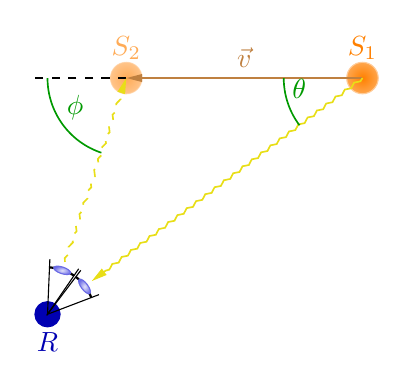
\begin{tikzpicture}
    \coordinate (R) at (0,0);  % Receiver position
    \coordinate (S1) at (4,3);  % Source position (initial)
    \coordinate (S2) at (1,3);  % Source position (point of reception)

    % -- Calculate angles as \Delta y/\Delta x
    \pgfmathsetmacro{\tiltone}{atan(3/4)}% Between R and S1
    \pgfmathsetmacro{\tilttwo}{atan(3/1)}% Between R and S2


    % -- Receiver (with telescope)
    \draw[receiver] (R) circle(0.16) node[below=3] {$R$};

    \begin{scope}[rotate=\tiltone]
        \telescope
    \end{scope}
    
    \begin{scope}[rotate=\tilttwo]
        \telescope
    \end{scope}


    % -- Source
    \draw[source] (S1) circle(0.2) node[above=3, orange] {$S_1$};
    \draw[source, opacity=0.66] (S2) circle(0.2) node[above=3, orange] {$S_2$};

    \draw[->, semithick, brown] (S1) -- (S2) node[midway, above] {$\vec{v}$};

    
    \draw[light] (S1) -- (\tiltone:\lt);  % Light Ray

    % -- Angles
    \def\angrad{1}

    \draw[angle] (S1) ++ (-180+\tiltone:\angrad) arc(-180+\tiltone:-180:\angrad) node [midway, above right=-2] {$\theta$};

    % \draw[dashed] (S2) -- (\tilttwo:\lt);
    % \draw[dashed] (R) -- (S2) --++ (-1.2*\angrad,0);
    \draw[dashed] (S2) --++ (-1.2*\angrad,0);
    % \draw[light, dashed] (R) -- (S2);
    \draw[light, dashed, shift={(R)}] (\tilttwo:\lt) -- (S2);  % If second telescope is whon
    \draw[angle] (S2) ++ (-180+\tilttwo:\angrad) arc(-180+\tilttwo:-180:\angrad) node[midway, above right=-2] {$\phi$};
\end{tikzpicture}


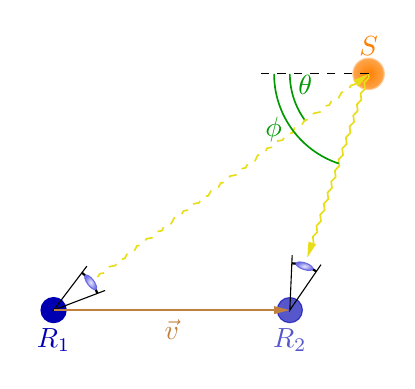
\begin{tikzpicture}
    \coordinate (S) at (4,3);  % Source position
    \coordinate (R1) at (0,0);  % Receiver position (initial)
    \coordinate (R2) at (3,0);  % Receiver position (point of reception)

    % -- Calculate angles as \Delta y/\Delta x
    \pgfmathsetmacro{\tiltone}{atan(3/4)}% Between R1 and S
    \pgfmathsetmacro{\tilttwo}{atan(3/1)}% Between R2 and S


    % -- Receiver (with telescope)
    \draw[receiver] (R1) circle(0.16) node[below=3] {$R_1$};
    \begin{scope}[shift={(R1)}, rotate=\tiltone]
        \telescope
    \end{scope}

    \draw[receiver, opacity=0.66] (R2) circle(0.16) node[below=3] {$R_2$};
    \begin{scope}[shift={(R2)}, rotate=\tilttwo]
        \telescope
    \end{scope}

    \draw[->, semithick, brown] (R1) -- (R2) node[midway, below] {$\vec{v}$};


    % -- Source
    \draw[source] (S) circle(0.2) node[above=3, orange] {$S$};
    

    % \draw[light] (S) -- (R2) ++ (\tilttwo:\lt);  % Light Ray
    \draw[light,shift={(R2)}] (S) -- (\tilttwo:\lt);  % Light Ray -> trick with shift is that (S) is unaffected by it

    % -- Angles
    \def\angrad{1}

    \draw[angle] (S) ++ (-180+\tiltone:\angrad) arc(-180+\tiltone:-180:\angrad) node [midway, above right=-2] {$\theta$};

    \def\angrad{1.2}
    % \draw[dashed] (R1) -- (S) --++ (-1.2*\angrad,0);
    \draw[dashed] (S) --++ (-1.2*\angrad,0);
    \draw[light, dashed, shift={(R1)}] (\tiltone:\lt) -- (S);
    \draw[angle] (S) ++ (-180+\tilttwo:\angrad) arc(-180+\tilttwo:-180:\angrad) node[midway, left] {$\phi$};
\end{tikzpicture}


\end{document}